\svnkwsave{$RepoFile: siminos/spatiotemp/chapter/lit.tex $}
\svnidlong {$HeadURL: svn://zero.physics.gatech.edu/siminos/spatiotemp/chapter/lit.tex $}
{$LastChangedDate: 2020-04-19 01:28:36 -0400 (Sun, 19 Apr 2020) $}
{$LastChangedRevision: 6820 $} {$LastChangedBy: predrag $}
\svnid{$Id: lit.tex 6820 2019-03-28 03:43:43Z predrag $}

\chapter{Spatiotemporal literature}
\label{chap:spatTempLit}

\begin{bartlett}{
\HREF{https://soundcloud.com/the-story-collider/kaca-bradonjic-the-nature-of-space-and-time}
{The Nature of Space and Time}
                }\bauthor{
Ka\'ca Bradonji\'c
                }
\end{bartlett}

\section{Spatiotemporal rocket science}
\label{sect:SpatTempRocketSci}

\begin{description}
\item[2017-01-23 Predrag]
not sure where to put this - into pipe blog or here, but
Wang \etal\rf{WGBGQ13}
{\em Towards scalable parallel-in-time turbulent flow simulations}
introduces ``the least squares shadowing (LSS) method'' and
uses \KS\ to illustrate the power of their method: ``
The initial condition is relaxed and information is allowed to propagate
both forward and backward in time. [...]
next-generation simulation paradigm can likely be spacetime parallel
simulations. These simulations subdivide the four-dimensional spacetime
computational domain. Each computing core handles a contiguous subdomain
of the simulation spacetime. Compared to subdivision only in the
three-dimensional space, spacetime parallel simulations can achieve
significantly higher level of concurrency, and reduce the ratio of
inter-core communication to floating point operations. [...]
Efficient time domain parallelism can only be achieved through
reformulating turbulent flow simulation into a well-conditioned problem.
We reformulate turbulent flow simulation into a well-conditioned problem
by relaxing the initial condition.
 [...]
Instead of trying to find the flow solution that satisfies both the
governing equation and the initial condition, we aim to find a flow
solution satisfying only the governing equation.
 [...]
Stability of the trajectory with a relaxed initial condition is achieved
by splitting a perturbation into stable and unstable components, and
propagating their effects forward and backward in time, respectively.
''

Blonigan and Wang\rf{BloWan14,BloWan15,BloWan16} might also be of interest.

\item[2017-01-25 Evangelos] In the sense that you describe in the last paragraph,
hasn't dynamics been dead already since Poincar\'e and Lorenz?
I mean that they showed that we have to study geometry and then time becomes
irrelevant. It's more like ``Dynamics is dead, long live dynamics!''

Wang \etal\rf{WGBGQ13} is very interesting indeed. I find it very similar
to your variational method for finding periodic orbits~\rf{CvitLanCrete02,lanVar1}.
In G.~Sanchez-Arriaga \etal\rf{sanchez2015} we have developed (without much thinking)
a boundary value solver discretized with finite differences both in time
and in space in order to detect periodic orbits. It resulted in a sparse
linear algebra system that was parallelizable, but we didn't study
how performance scales. There should be a straightforward extension of
Wang \etal\rf{WGBGQ13} for periodic orbits.

The main two challenges that I see with methods such as the
above~\refrefs{CvitLanCrete02,lanVar1,sanchez2015,WGBGQ13} is 1) finding
a suitable initial guess and 2) increased memory requirements. The first one
is there already when we search for periodic orbits and I suspect that it will
be worse for turbulence simulations. The second one might not be as serious
in next generation HPC platforms.

\PCpost{2017-03-09}{
Andrej Junginger, J\"org Main, G\"unter Wunner and Rigoberto Hernandez,
{\em Variational principle for the determination of unstable periodic orbits
  and instanton trajectories at saddle points},
\arXiv{1703.02472}
(Prof. Uzer knows the authors well) write: ``
  The complexity of arbitrary dynamical systems and chemical reactions, in
particular, can often be resolved if only the appropriate periodic orbit - in
the form of a limit cycle, dividing surface, instanton trajectories or some
other related structure - can be uncovered. Determining such a periodic orbit,
no matter how beguilingly simple it appears, is often very challenging. We
present a method for the direct construction of unstable periodic orbits and
instanton trajectories at saddle points by means of Lagrangian descriptors.
Such structures result from the minimization of a scalar-valued phase space
function without need for any additional constraints or knowledge. We
illustrate the approach for two-degree of freedom systems at a rank-1 saddle
point of the underlying potential energy surface by constructing both periodic
orbits at energies above the saddle point as well as instanton trajectories
below the saddle point energy.
}

\NBBpost{2014-11-15,2017-01-26}{
Fazendeiro, Boghosian, Coveney and L{\"a}tt\rf{FBCL10}
{\em Unstable periodic orbits in weak turbulence}
seem to have applied the variational periodic orbit finding method to fluid
flow by parallelizing the whole thing.
    }

\PCpost{2017-05-05}{
Boghosian \etal\rf{BFLTC11} {\em New variational principles for locating
periodic orbits of differential equations} is
the most detailed discussion (see also \refrefs{BBLTFC11,FBCL10}):

They reformulate the space–time algorithm of Lan and
Cvitanovi\'c\rf{lanVar1} in a clear-headed way, and use
using the methods of gradient descent or conjugate
gradients to solve the variational equations.

They apply it to the lattice-Boltzmann method for the solution of the
Navier–Stokes equations, with a fully parallel implementation using the
Message Passing Interface.
The method has first been tested on the Lorenz equations\rf{BBLTFC11}.
They apply this to weak homogeneous turbulence driven by an
Arnold–Beltrami–Childress force field in three spatial dimensions. Because
the algorithm requires storage of the space–time lattice, even the smallest
orbits require resources on the order of tens of thousands of computing
cores. Using this approach, two UPOs have been identified and some of their
properties have been analysed.

In \refref{FiBoKo05} they discuss ``Ginzburg–Landau-type minimization.''
(Probably not worth pursuing, they do not return to it)

''    }

\MNGpost{2017-08-16}{:
%\begin{description}\item[2017-01-23 Predrag]
Discussed David Lasagna's paper\rf{Lasagna17} on time averages and their
sensitivity to parameters. PC brought up the fact that derivatives of
averages tend to be fractal in nature due to horseshoes?
}

\item[2017-08-16 Ashley, 2019-02-21 Predrag]
Davide Lasagna\rf{Lasagna17}
{\em Sensitivity analysis} {\em of turbulence using unstable periodic orbits:
a demonstration on the {Kuramoto-Sivashinsky} equation}.
\\
{\bf  Ashley}
\Po s are finite, so can compute sensitivity avoiding the time integral.

Sets up a Lagrangian depending on parameters, takes variational derivative

ends up with the adjoint equation

(8b) is not a condition, it is fact.

Lasagna, Sharma and Meyers\rf{LaShMe18} {\em Periodic shadowing sensitivity
analysis of chaotic systems}, \arXiv{1806.02077} is a continuation of
Wang\rf{Wang13,Wang14}. The find Wang\rf{Wang13} Shadowing Lemma a major advance.
They credit Lasagna\rf{Lasagna17} for ``deriving periodic boundary conditions in
time for the sensitivity equations.''
The contribution of \refref{LaShMe18} is a shadowing-based algorithm, based on
the idea of enforcing periodic boundary condition in time to the sensitivity
equations, leading to the time periodic shadowing. Providing such boundary
conditions directly not only results in a method that is potentially simpler, but
it sufficient to obtain bounded (periodic) solutions almost always, resulting in
accurate gradients.

The adjoint periodic shadowing method we employ a classical Lagrangian
approach\rf{Cacuci81,BorSch11} starts by constructing the finite-time Lagrangian
function (16).

``Sum-of-squares" papers (seem unrelated to the spatiotemporal effort):

Huang, Chernyshenko, Goulart, Lasagna, Tutty and Fuentes\rf{HCGLTF15}
{\em Sum-of-squares of polynomials approach to nonlinear stability of
fluid flows: an example of application}

Lasagna, Huang, Tutty and Chernyshenko\rf{LHTC16}
{\em Sum-of-squares approach to feedback control of laminar wake flows}

Huang,  Jin,  Lasagna,  Chernyshenko and Tutty\rf{HJLCT17}
{\em Expensive control of long-time averages using sum of squares and its
application to a laminar wake flow}


The ``adjoint periodic shadowing methods'' papers are rather tedious read (lots of
variational equations!):

Cacuci\rf{Cacuci81} {\em Sensitivity theory for nonlinear systems. {I. Nonlinear}
functional analysis approach} is cited by many authors up to 2019, with suggestive
paper titles, like

Luchini and Bottaro\rf{LucBot14} {\em Adjoint equations in stability analysis}

Cacuci\rf{Cacuci15} {\em Second-order adjoint sensitivity analysis methodology
(2nd-{ASAM}) for computing exactly and efficiently first- and second-order
sensitivities in large-scale linear systems: {I. Computationa}l methodology}

Cacuci\rf{Cacuci19} {\em Second-order sensitivities of a general functional of
the forward and adjoint fluxes in a multiplying nuclear system with source}:
\\
2nd-order (Hessian) sensitivity information accelerates the
convergence of optimization algorithms.
\\
In atmospheric
sciences ``second-order adjoint
models" were used to compute products between the Hessian of the cost
functional and a vector (representing a perturbation in sensitivity analysis, a
search direction in optimization, an eigenvector, etc.) to perform sensitivity
analysis of the cost function with respect to distributed observations.

\item[2017-02-05 Tobias Schneider]  <tobias.schneider@epfl.ch>
There were several talks about these topics at
\HREF{http://www.pasc16.org} {pasc16.org}. In a session I organised Diego
Donzis gave an exciting talk about fluid dynamics simulations in the
future. Donzis and Aditya\rf{DonAdi14}
{\em Asynchronous finite-difference schemes for partial differential equations}
   is one of the papers but there is a lot of unpublished stuff.

Check MS14 at \HREF{http://www.pasc16.org/program/program/}
{pasc16.org/program} for Donzis abstract:
``
Turbulence is the most common state of fluid motion in nature and
engineering and is critical in environmental, astrophysical and
engineering flows. However, the complexity of the governing equations
leads to wide ranges of temporal and spatial scales and render the
problem almost intractable analytically. Thus, simulations, in particular
direct numerical simulations (DNS) which resolve the entire range of
scales from the exact governing equations, have become an indispensable
tool to advance the field. While very accurate spectral methods have been
used extensively up to petascale levels, they typically require
collective communications and synchronizations, two well-known potential
bottlenecks at exascale. We present our recent work on novel asynchronous
numerical schemes that virtually remove computational obstacles at a
mathematical level and present a path towards exascale DNS of turbulent
flows. We will highlight implications, challenges and opportunities in
terms of numerical issues, parallel performance, and implementation
issues on future exascale systems.
''

\item[2019-03-19 Tobias update]
I haven't seen any further developments beyond what Diego Dozis was
talking about but I am also not following the field too closely. These
developments are moreover aimed at something less exciting than treating
space and time on an equal footing. The idea is: How to relax the
requirement that all CPUs in a large computer have to work in a perfectly
synchronised way. This leads to numerical time-marching schemes for which
the individual CPU cores can work asynchronously. It's a big question
that arises with modern computers with literally thousands of CPU cores.
Essentially the idea is that you split the spatial domain and
time-integrate this domain independently of the others. When one needs
info on the neighbouring domains (typically at the boundaries) one does
not insist that the data for all subdomains is given at exactly the same
time step. Of course that leads to small errors but those integration
errors can be controlled. It's really just about time-marching schemes
that pose fewer synchronisation constraints and are thus better suited
for huge computers where inter-CPU communication is expensive.

I think numerical schemes that truly appreciate that space and time are to be
treated together will be on us and our community.

I have a few ideas that I would love to discuss. We are working on
constructing a variational code for Navier-Stokes (matrix-free). We will
start with a \KS\ demonstration (by the early fall?) and then move to 3D
Navier-Stokes.

My plan is to develop \emph{variational adjoint methods}\rf{Schneider19}.

\emph{Machine learning} will be used for constructing initial guesses.

Matrix-free adjoints\rf{Faraz15}.

Setup for 3D Navier-Stokes: combine parallelized Channelflow 2.0
with a robust, variational tool
for computing periodic orbits of 3D flows.

Historically, guesses are extracted from approximate recurrences observed
in long turbulent simulations\rf{pchaot}. This is
inefficient, useful only for the short, least unstable orbits.

\PCpost{2017-09-04} {               \toCB
Junginger \etal\rf{JuMWuHe17} {\em Variational principle for the determination
of unstable periodic orbits and instanton trajectories at saddle points} seem
specific to Hamiltonian dynamics. They write:

The complexity of arbitrary dynamical system  (chemical reaction, in
particular) can often be resolved if only the appropriate periodic orbit - in
the form of a limit cycle, dividing surface, instanton trajectories, or some
other related structure - can be uncovered. We present a method for the
direct construction of unstable periodic orbits and instanton trajectories at
saddle points by means of Lagrangian descriptors. Such structures result from
the minimization of a scalar-valued phase-space function without the need for
any additional constraints. We illustrate the approach for two-degree of
freedom systems at a rank-1 saddle point of the underlying potential-energy
surface by constructing both periodic orbits at energies above the saddle
point as well as instanton trajectories below the saddle-point energy.

Check also
Jim{\'e}nez Madrid and Mancho\rf{JimMan09}
{\em Distinguished trajectories in time dependent vector fields}:
Fixed points and periodic orbits are keystones for describing solutions of
autonomous and time periodic dynamical systems, as the stable and unstable
manifolds of these hyperbolic objects form the basis of the geometrical
template organizing the description of the dynamical system.
They give a new definition of ``distinguished trajectory'' that
encompasses the concepts of fixed point and periodic orbit and which when
applied to finite time and aperiodic dynamical systems identifies special
trajectories that play an organizing role in the geometry of the flow.
The definition is valid for identifying distinguished
trajectories with hyperbolic and nonhyperbolic types of stability. The
definition is implemented numerically and the procedure consists of
determining a path of limit coordinates. In the context of highly
aperiodic realistic flows the definition characterizes distinguished
trajectories in finite time intervals, and states that outside these
intervals trajectories are no longer distinguished.
}

\PCpost{2017-11-03} {
\HREF{https://scholar.google.com/citations?hl=en&user=6pzhrnkAAAAJ}{Jianke
Yang}\rf{Yang15} {\em A numerical method for computing time-periodic solutions
in dissipative wave systems} is another paper that finds \KS\ and \cGL\ {\rpo}s
using spatiotemporal methods.

It looks quite interesting, but it will requires bit of work to understand the
paper. Yang's Matlab codes are available
\HREF{http://www.cems.uvm.edu/~jxyang/codes.htm} {online}, so one can download
his \KS\ code and give it a go on some of our solutions.
    }

\item[2019-02-06 Predrag]
Catching up on the more recent work of
\HREF{https://scholar.google.com/citations?user=lOmH5XcAAAAJ&hl=en&oi=sra}
{Patrick Blonigan} (who happens to be recent Farazmand coauthor :)
and
\HREF{https://scholar.google.com/citations?user=DG3w3kMAAAAJ&hl=en&oi=sra}
{Qiqi Wang}.

Wang\rf{Wang13}
{\em Forward and adjoint sensitivity computation of chaotic dynamical systems}
has 44 citations.
It uses Lyapunov eigenvector decomposition for sensitivity analysis, but
that has high computational cost when the dynamical system has many
positive Lyapunov exponents.

Blonigan and Wang\rf{BloWan13}
{\em Multigrid-in-time for sensitivity analysis of chaotic dynamical systems}:

Wang\rf{Wang14} {\em Convergence of the least squares shadowing method for
computing derivative of ergodic averages}

Their papers say that LSS was introduced in
Wang, Hu and Blonigan\rf{WaHuBl14} {\em {Least Squares Shadowing} sensitivity
analysis of chaotic limit cycle oscillations}. The paper has 42 citations.
%, many of which are self-citations.

LSS computational cost is $O(mn^3)$ where $m$ is the number of time steps, and
$n$ is the number of dynamical degrees of freedom.

When the dynamical system is high dimensional, e.g., a discretized
partial differential equation, iterative solution methods should be used
instead of direct matrix solvers. Because the system is well-conditioned
and only twice as large as an initial value problem, an iterative
solution can potentially cost only a small multiple of an initial value
solution.

What I do not get is
the cost function - it is usual squares, but with respect to a
``pre-specified reference trajectory.''

\emph{Sensitivity analysis}\rf{LeAlHa00} computes the derivative of outputs to inputs
(derivative with respect a control parameter) of a
simulation. Conventional methods, including the tangent and the adjoint method,
fail when the dynamical system is chaotic and the outputs are long time averaged
quantities.

ensemble adjoint method\rf{LeAlHa00}

\index{sensitivity!analysis}

Chater \etal\rf{CNBW17} {\em Least squares shadowing method for sensitivity
analysis of differential equations}

Chater, Ni and Wang\rf{ChNiWa17} {\em Simplified {Least Squares Shadowing}
sensitivity analysis for chaotic {ODEs} and {PDEs}}

Blonigan and Wang\rf{BloWan18} {\em Multiple shooting shadowing for sensitivity
analysis of chaotic dynamical systems} present a variation of the method suitable
for high-dimensional systems, using multiple-shooting strategies.

Craske\rf{Craske19}
{\em Adjoint sensitivity analysis of chaotic systems using cumulant truncation}

Blonigan\rf{Blonigan17} {\em Adjoint sensitivity analysis of chaotic dynamical
systems with non-intrusive least squares shadowing} introduces a ``non-intrusive
least-squares shadowing (NILSS)'' algorithm.

Ni and Wang\rf{NiWan17} {\em Sensitivity analysis on chaotic dynamical systems by
{Non-Intrusive Least Squares Shadowing ({NILSS})}}

Ni\rf{Ni19} {\em Hyperbolicity, shadowing directions and sensitivity analysis of
a turbulent three-dimensional flow} uses the NILSS algorithm.

Kim and H. Choi\rf{KimCho14}
{\em Space-time characteristics of a compliant wall in a turbulent channel flow}

\PCpost{2019-03-19} { {\bf to Matt}
One of our problems is that we do not know what our spatiotemporal
variational method is called by other people who have presumably already
crossed this bridge before us.

In \HREF{http://www.inpe.br/ccis2019/} {\em CCIS 2019}
{\em Conference of Computational Interdisciplinary Sciences}
% President's room, Bobby Dodd Stadium, should be of interest to us:
\HREF{https://mae.mst.edu/academy/pepper} {Darrell Pepper}
gave a pleasant engineering talk to non-specialist audience on his
``meshfree approach.''
% March 19 10:30-11:30,
He has have been at this for a while, but is still active. His students
use the method in fluid dynamics problems. He tells many jokes, like
older professors from Las Vegas tend to. Sometime. His claims to fame are many, but in
particular he computed the direction of the radioactive plumes for both
3-Mile Island and Chernobyl.
% See whether you can chat him up, and show him your poster (illegally,
% like in a Moroccan bazaar, as an unregistered poster perhaps:).
% Curiously, not one other talk or poster seems of interest to us.

Most recently, Pepper has been working on how to
equip Las Vegas firemen with real time info which way the plumes are going, see
Pepper and Gonzalez\rf{PepGon18} {\em A localized meshless technique for
generating {3-D} wind fields}. For us Sect.~4. {\em The Meshless Method} is
helpful, as a succint summary. The point there is that they replace a
square mesh by support on a set of irregularly placed points (for
example, Las Vegas firehouses). Few bullet points from his talk

\begin{enumerate}
  \item
boundary element methods reduce the problem by one dimension (boundary
instead of the bulk)
  \item
Local Petrov-Galerkin good for steep gradients, \ie, shocks
  \item
Mashless methods work for Navier-Stokes, heat transfer, etc. They work
with primitive equations (velocity fields) rather than with vorticities,
as boundary conditions are difficult in the vorticity formulations.
  \item
Multiquadrics are good as they have explicit expressions for derivatives
  \item
Global mashless equation (linearized?) is a large matrix equation.
It can suffer poor conditioning, and is
efficient only for square domains.
  \item
Local mashless methods loop through all points one by one. They are
not ill conditioned.
  \item
They are engineers, they are happy if solutions are good to a few \%.
  \item
FreeFEM finite element code is free and can be downloaded
  \item
In atmospheric simulations: minimize variance between the observed and
the computed.
  \item
My feeling: meshless methods are good for inhomogenous discretizations, funky
boundary conditions. In our case, spectral methods (Fourier represenatations)
probably work better.
\end{enumerate}

The rest is my reading.
The meshless method was introduced by Fasshauer\rf{Fasshauer02} from whom
I gleaned this:

    They are interested in the numerical solution of a generic nonlinear
    (elliptic) PDE as a boundary value problem on some domain. Instead of
    discrete meshes, they work with the globally supported radial basis
    function (RBFs). Not clear to me how well these bases can be used on
    periodic domains. Globally supported multiquadric radial basis
    functions can be used for Newton iteration numerical solution of
    nonlinear partial differential equations. The use of coarse meshes
    during the initial iterations along with a multiquadric parameter
    which is adjusted with the meshsize increases the efficiency and
    stability of the algorithm.

    Fasshauer\rf{Fasshauer02} ``test problem'' is a nonlinear elliptic
    (\ie, a single $2D$ Laplacina) PDE on a unit square, different from
    but not totally irrelevent for our \KS\ application: he computes what
    we would call solution $u(t,x)$ over a quadratic domain, compatible
    with the given PDE. His solutions are of much simpler shape than most
    of Matt's solutions, so Matt seems to be solving a harder problem.

If of interest, try to check out the Fasshauer book\rf{Fasshauer07} with MATAB
codes.
Maybe we also have to learn about ``Nash iteration'' and the
Kansa\rf{KansaI90,KansaII90} or ``multiquadric method'' for solving problems in
2D and 3D arbitrary domains. Engineers like it for applying it to inhomogeneous
and irregular complex geometries. Closer to home, it has been used for computing
solutions to Burger's equation\rf{GaoChi14,SarAmi14}.

    }

\end{description}

\subsection{Adjoint sensitivity analysis}
\label{sect:AdjSenAn}

Sensitivity analysis, according to
\HREF{https://docs.juliadiffeq.org/latest/analysis/sensitivity.html}
{Julia}:

The local sensitivity of a solution of an ODE or a PDE model is given by the
derivative of the $i$th independent field of the solution with respect to the
$j$th parameter,
\( {\pde u_i}/{\pde p_j}. \)
There are three types of sensitivity analysis.
Local forward sensitivity analysis gives the gradient of the solution  along the
time evolution with respect to a parameter.
Local adjoint sensitivity analysis gives the gradient of some
functional of the solution, such as a cost function.
Global sensitivity analysis methods computes the
sensitivity over a domain without calculating derivatives.

Adjoint sensitivity analysis is used to find the gradient of the solution
$x(t,p)$ with respect to some functional of the solution. This adjoint requires
the definition of a scalar observable $a(x)$ where $x$ is a solution to the
differential equation.
Adjoint sensitivity analysis finds the gradient of
the integrated observable
\beq
A^t (x_0,p) = \int_{0}^{t}d\tau a(x(\tau,p)),
\ee{ASintObs}

I also like this
\HREF{https://marcschwalbach.com/posts/2016/5/29/a-taste-of-adjoint-sensitivity-analysis}
{introduction} by Marc Schwalbach. Unfortunately he lost steam after one post :)
For a weatherman's angle, see
Errico\rf{Errico97} {\em What is an adjoint model?}.


Traditional adjoint sensitivity methods face fundamental limitations when applied
on turbulence, which are addressed by development of robust methods for adjoint
analysis\rf{WaHuBl14}. %[15].

Over the past two decades it has been established that the
numerically exact invariant solutions of the Navier-Stokes
equations (``recurrent flows") serve as the ``building blocks" that
shape turbulent dynamics.

This dynamical framework  will be used to solve (and design) turbulent drag
reduction and optimisation problems in turbulence, in particular design of
compliant surfaces for drag reduction in plane channel flow.

Lasagna and Sharma are developing so called adjoint-based variational methods for
sensitivity analysis. With sensitivity information, they can design optimal
drag-reducing surfaces by using gradient-based optimisation methods.

The existing periodic orbit theory, so far successfully applied
only to low-dimensional dynamical systems, posits that the
description of the chaotic / turbulent state space is given by
ensembles of hierarchically organised unstable period solutions of
increasing length.
In contrast, Lasagna's working hypothesis is that a few periodic orbits of long
periods, embedded in state-space regions most frequented by turbulence and thus
capturing the full range of dynamical events, suffice. Which strategy works best
in practice remains an open question, and the approach proposed here should
certainly be explored.

They plan to develop new space-time parallel numerical methods to
find periodic orbits with long period and then develop adjoint
solverss
(formulated as a boundary value problem with periodic boundary condition)
to obtain gradient information.

The approach is based on the idea that adjoint analysis of such
structures can provide accurate sensitivities of time averaged
quantities with respect to the design surface parameters.


The proposed adjoint approach offers the ability to obtain
gradient information
with respect to a large number of parameters (the spatial
distribution of material properties)

For small perturbations, the sensitivity of a system is given by
the gradient with respect to a parameter.
Lasagna and Sharma have shown that this gradient can be obtained by
adopting adjoint techniques to periodic orbits.

A variation of any of the system's parameters (the viscosity in
case of {Kuramoto-Sivashinsky}) produces a computable state-space
distortion of periodic trajectories. They illustrate this by
varying viscosity $\nu$ from $(2\pi/39)^2$ to $(2\pi/38.5)^2$
for their shortest periodic orbit.

They compute a few thousand periodic orbits of period $\simeq 1000 \nu$. The
question is: what is the right orbit to use?

    \PC{2019-03-19} {It is Japanese heresy all over again (see comments at the
                     end of this section)}
They plan to consider only one periodic orbit, having a sufficiently long period
such as to span all possible dynamical events encountered by long chaotic
trajectories, i.e. shadowing many shorter, more elementary recurrent structures.
This is a different direction, where long-period orbits capture statistics of
turbulence.
The approach is based on empirical evidence
that, at least for low dimensional systems, the
variability across periodic orbits of similar
period $T$, e.g. the standard deviation of distribution
follows
the central limit theorem and decreases as
$1/\sqrt{T}$.

They view
turbulent flows as stationary equilibria of a four-dimensional PDE,
the Navier-Stokes equations in three spatial directions plus time,
with periodic conditions in time justified by the invariance under
time translation of statistically developed flows. With
sufficiently long temporal domains (akin to spatial domains larger
than a minimal flow unit), they expect that averages and their
gradients will converge with the size of the temporal domain.

Their goals are to a) demonstrate that these \po s
exists in Navier-Stokes problems b) develop an
understanding of their significance in describing turbulent
structure and evolution, b)
formalise a framework for control and optimisation of turbulence.

{\bf Time-parallel methods for long orbits}
They plan to develop new computational methods, suitable for arbitrarily long
orbits.

The system arising in the Newton search iterations is the
adjoint of this.
The
global-in-time nature of the adjoint problem on periodic orbits
enables mixed space/time domain decomposition methods, to
distribute computation across independent nodes of a
distributed memory system.

They use multiple-shooting techniques, exploiting time as an
additional direction for distributed memory parallelism. The
approach consists in partitioning the temporal interval into
independent sub-domains and than seeking the terminal adjoint
solution at the shooting points, imposing that the solution is
globally periodic and continuous at the shooting points.
    \PC{2019-03-19} {Just to drive Predrag more bewildered, they plot time
                     horizontally, space vertically :)}

Matrix-vector products for the construction of the Krylov basis
vectors in the GMRES solver can now exploit the block-banded
structure of this problem, by distributing the
sub-matrix/sub-vector products to different computational nodes in
a time-parallel fashion, and using independent adjoint
time-steppers to calculate actions, with minimal communication
required. Mixing spatial/temporal parallelism, via processor
grouping routines is a natural
extension.

Even if the proposed approach based is likely not applicable to
high-Reynolds number flows, the work holds the potential to accelerate
future development of adjoint methods suitable for chaotic systems\rf{LaShMe18}. % [16].


Task A.1 – This will be based on in-house codes under development at Southampton and
freely available software (e.g. J Gibson's channelflow). The influence of
the compliant wall will be modelled by linearised kinematic boundary
conditions, using standard modelling procedures\rf{LuShMc16,KimCho14}. % [12,7,11].


{\bf Space-time parallel algorithms for long periodic orbits.}

A dedicated c++ parallel Krylov
subspace library being developed at Southampton
\HREF{https://github.com/gasagna/ParK} {gitHub.com/gasagna/ParK}. The
Newton-Krylov-hookstep\rf{Visw07b} % [14]
approach will be used. They will
initially rely on temporal parallelism and subsequently extend the
library to spatial parallelism.

{\bf Space-time parallel adjoint solver.}
We will then couple
the adjoint time steppers developed in B.1 with the available
parallel Krylov solver to solve the adjoint boundary value problem.


The intersection of recurrent flow analysis with adjoint
techniques for optimisation is largely unexplored. So far,
recurrent flows have been primarily used as a proxy to understand
dynamics, i.e. as an analysis tool. Their program is
complementary to our efforts, because they aim to employ these
ideas for control and design.

\bigskip

On {\bf Japanese Heresy},
from \texttt{dasbuch/book/chapter/recycle.tex}:
\begin{description}
\item[2011-11-15  Predrag]%\item[2007-11-28 Predrag: Japanese Heresy]
Then there is in literature an `Alternative Periodic Orbit Theory' so
bold that one can only call it The Heresy: the conjecture is that if
one looks carefully enough, there exists a \emph{single} \po\ that
captures all dynamical averages of a turbulent flow. This is so wrong
that one is at loss what to say: there is NO such single \po.
Instead, there is the well established theory that says how \po s are
to be used, and how many are needed to capture the hyperbolic parts
of the {\nws} to a desired accuracy. It is as elegant and systematic
as Statistical Mechanics and Quantum Field Theory. Read
\HREF{http://chaosbook.org/}{ChaosBook.org}. But who reads books
nowadays?

Of course, if one picks at random a very long \po, one will get
estimates as good as from an ergodic trajectory of comparable length,
but then why make life hard by insisting on exact recurrence? When one
starts out, The Heresy is one of the paths to enlightenment: Berry
diplomatically writes ``he found one orbit'' in a pean to
Gutzwiller\rf{Berry12}. Indeed, in Gutzwiller first paper
(1969) on anisotropic Kepler system,  the \emph{one} \po\ obtained by
adiabatic deformation of a Kepler ellipse yielded 10\%\ accuracy,
which was great, as in those days it was generally believed that
semiclassics should be bad for the ground state. Two years later
Gutzwiller invented periodic orbit theory as a tool for physicists,
applied it to the full anisotropic Kepler problem, and since then
there is no turning back. Similarly, Kawahara\rf{KawKida01}
computed the first Navier-Stokes \po\ solution embedded in turbulence,
and observed that it gave rather accurate estimates of observables
such as the dissipation rate.
\end{description}



From \texttt{siminos/blog/UPO.tex}:
\begin{description}
\item[2012-05-13  Predrag] [...] until the first unstable periodic solutions of
Navier-Stokes were computed by Kawahara and Kida\rf{KawKida01} in 2001,
determining such solutions seemed utterly out of reach. Their \pCf\
`upper' periodic orbit appears embedded in the turbulent sea, and
captures statistics so well that it lead to the `Heresy', a belief of the
innocent that there exists a \emph{single} periodic orbit (!) that
captures turbulent statistics; we do not cite these papers, as
that was a vain hope of those too busy to read ChaosBook.org.

\item[2011-11-15  Predrag] From \texttt{pipes/blog/Alabama.tex}:
\\
Can you try this?
Compute the averages for $(D(\zeit),I(\zeit))$ for one period of
$\RPO{36.92}$ and for your $S$-subspace turbulent trajectory. That should
yield two point on the diagonal.  Kawahara was lucky there - they were
unreasonably close, the root of the Japanese Heresy. If they are not close,
$\RPO{36.92}$ does not go through the most concentrated regions of natural
measure.

From \refref{SCD07}: ``
Similarly close prediction of mean dissipation rate in the
\pCf\ from a single-period \po\ computed by
Kawahara and Kida\rf{KawKida01} has lead to
optimistic hopes that `turbulence' is different from
low-dimensional chaos, insofar that the determination of one special
\po\ could yield all long-time averages.
Regrettably, not true -- as always, here too one needs a hierarchy
of \po s of increasing length to obtain accurate
predictions\rf{DasBuch}.
    ''


\item[2007-11-28 Predrag: Japanese heresy]
We do not want to refer to wrong papers, but here it is, for
the internal record, so we do not forget not to cite it:

Mitsuhiro Kawasaki and Shin-ichi Sasa\rf{KaSa05},
    ``Statistics of unstable periodic orbits of a chaotic dynamical system
    with a large number of degrees of freedom.''

\item[2012-08-12  Predrag]
Goldobin\rf{Goldobin12} \emph{Limit distribution of averages over
unstable periodic orbits forming chaotic attractor}, \arXiv{1208.1691},
is much weirder still: it is motivated by the Japanese Heresy and cites
only the Maryland non-theory paper as the source on the periodic orbit
theory.  Remind him to cite ChaosBook.

\end{description}

From \texttt{siminos/lyapunov/Henon.tex}:
\begin{description}
\item[2011-10-06 Kazz]
There should be many \po s flowing like the chaotic trajectory. They
therefore have long periods and are non-hyperbolic (almost, always). But,
in my view, it would be interesting to decompose properties of the
chaotic trajectory into those of only a few number of \po s, whose period
is rather short and thus each of which covers only a local region of the
attractor. For the H\'enon map, we are still lacking such a minimal \po,
which accounts for the remaining non-hyperbolic points of the chaotic
trajectory.

\item[2011-10-06 Predrag]
Wow! This comment makes no sense, but it does smack of the famous
Japanese Heresy. There is NO such thing -
instead of this there is perfectly well developed theory that says how
you use \po s and how many do you need to capture the hyperbolic parts of
the {\nws}.
\end{description}

\section{Spatiotemporal literature - a blog}
\label{sect:SpatTempLit}

\begin{description}

\MNGpost{2018-07-17}{

\textbf{Notes on Literature review in thesis proposal}
I tried to motivate the need to go spatiotemporal by the wall that's been
hit in pipe and channelflow while still celebrating the amount of work
that codes like \texttt{channelflow} and \texttt{openpipeflow} have been
able to accomplish. It probably comes off as arrogant and I need to
rewrite it but I'm trying to get the point across that: There are lots of
people stepping back and trying to find other paths to solving the issues
of high-dimensional systems because the direct approach is providing
diminishing returns.

Don't mind all of the names and bibtex references, it was just
brainstorming that I didn't remove.
     }

\PCpost{2018-07-21}{``Lots of people stepping back and trying to find other
paths?'' Only our Wednesday Hangout crowd has computed Navier--Stokes
\ecs s\ in small computational domains, and I'm not aware of anyone
thinking of ``other paths'' to computing \ecs s\ in spatially infinite
domains other than you and me. Looking forward to reading the literature
review of these many paths that I'm unaware of.
}

\MNGpost{2018-07-23}{
I meant more along the ideas of what people are to do after the small
computational domain calculations are exhausted, not that others are
attempting to explain infinite spatiotemporal domains. For instance, some
of the ``other paths" are looking for edge states, families of
self-similar solutions, investigating localized solutions, reduced-order
models using Koopman modes, Nigel Goldenfeld's predator-prey ideas. My
statement was merely attempting to describe the many branches of
turbulence research. They are unrelated to my project so I'll use the
excuse that this was just an expedient comment in my blog and not a deep
philosophical statement.
}


    \PCpost{2016-11-10}{
Sobolev norms we have pondered a lot (sprinkled through various blogs) but for
now stick to the L2 (AKA Euclidean) norm.

Papers to read, possibly to test your variational
    code on the soultions reported there:

Rempel\etal\rf{RCMR04} {\em Analysis of chaotic saddles in high-dimensional
dynamical systems: the {Kuramoto-Sivashinsky} equation}.
Only in the antisymmetric subspace $\bbU^+$, periodic on $2\pi$ and vary
hyper-viscosity $\nu$. Might be good - do not know. For some reason neither
Siminos nor Budanur nor Xiong seem to have looked at this paper, nor the
subsequent ones.

Saiki\etal\rf{SYCMR15} {\em Reconstruction of chaotic saddles by
classification of unstable periodic orbits: {Kuramoto-Sivashinsky} equation}:
they work only in the antisymmetric subspace $\bbU^+$, see their Eq.~(3), but are
periodic on $2\pi$ and vary hyper-viscosity $\nu$, so you'll have to convert.
Looks like cut and paste of their earlier \refref{RCMR04}.
They use the PIM triple method\rf{pimyk,ReCi05}. BTW, calling a \po\  UPO is
like saying ``I am riding unstable bicycle'' every time you get on a bike
(all bicycles are unstable): `Note that our notation ``a-UPO'' may sound
awkward when expanded as ``attractor-unstable periodic orbit.''' In all
fairness, stupider things are known, like ``nonchaotic orbit" instead of \po,
check the next cubicle :)

What is obvious from looking at a paper like this one is that spacetime
invariant 2-tori persist in continuous families, as one change the domain
size $L$, so that must mean an additional marginal direction eigenvector for
the torus-finding variational routine...

Croft's papers\rf{CroDav06,Crofts07thesis,CroDav09,CrDaGo16} probably use
pseudoinverse - Levenberg-\-Marq\-uardt described in an appendix of
\refref{SCD07} is might be an example.
    }

\MNGpost{2016-12-20}{
Read through half of Moser\rf{moser86}. It is indeed hard to read but I'm
hoping that in conjunction with de la Llave's \textit{Introduction to KAM
Theory} I will get something out of it.

Read through about a quarter more of Trefethen\rf{Trefethen97} as well as went to
the physical library to skim some texts that another student recommended
for me. They were math texts on par with Moser\rf{moser86} about functional
analysis.
Read some more of numerical linear algebra, Trefethen\rf{Trefethen97},
starting to enjoy it as I think it is written quite well.

% While interesting, I decided to leave in the library for the
% rainiest of days.
    }


\MNGpost{2017-05-05}{Read Boghosian \etal\rf{BFLTC11}.
        }

\MNGpost{2017-05-08}{
I was reading a number
of papers\rf{Meza95,Chu09,BroWal97,MiAK03} having to do with
ill-conditioned linear systems and how to circumvent issues with GMRES.
}

\MNGpost{2017-06-06}{
Read some Guckenheimer\refref{guckb}
}

\MNGpost{2017-09-05}{Read Junginger \etal\rf{JuMWuHe17}
{\em ez, “Variational principle for the determination of unstable periodic
orbits and instanton trajectories at saddle points}, I think it could possibly
introduce some important topics.
}

\MNGpost{2017-04-14}{ I've been reading a bunch of papers\rf{TBAMR92} on
preconditioning methods; and specifically for GMRES algorithm.
}

\MNGpost{2018-01-23}{
Browsed through arXiv to try to survey the recent literature in fluid dynamics and chaotic dynamics fields
just to try and branch out a little bit so that my world view isn't a single leaf of the forest. Trying
not to spend too much time with them, just skimming and reading abstracts until my curiosity is peaked.

Also rereading the cats' blog, and subsequent papers in depth so that I can attempt to be of some use to Han Liang. I find Predrag's
write-up about the relative action definitions that appeared in \refref{LiTom17b} to be much more understandable
than the actual paper, and am hoping to understand the spatiotemporal cat map definition version of the
relative action soon.

Recently checked out a book on spectral methods in fluid dynamics from the Gatech library, it's a secondary
read for sure but I find it useful in formalizing the ideas I have learned through coding.
}

\MNGpost{2018-02-12}{
Been reading the same texts as well as \refrefs{Lopez2015,MarWes01,BolTre10}.
    }

\MNGpost{2018-02-16}{
Read Mackay and Meiss\rf{MacMei83}. Even though its three pages I didn't
really understand the corollary where they prove that multipliers
corresponding to the stability of the second variation of the action
(because the first variation is by definition to be zero) are reciprocal
reals, past the point that they know that there is a matrix that can be
written in a certain way under certain circumstances
    }

\MNGpost{2018-02-16}{
Reading Lopez\rf{Lopez2015} 2015. It seems that what we're doing is very close to being identical except
the fact that I am allowing the spatial domain size to vary. In the appendices she also
notes that the best (among numerous different behaviors) convergence behavior was when she used GMRES
as well as a preconditioning matrix that is the inverse of the linear portion of the \jacobianM.
(The matrix of variations of the corresponding linear portion of the nonlinear algebraic equations),
so with that I would argue that what is being done on my front is \emph{only} different in the fact
that I am working with the \KSe\ and am allowing
the spatial domain size to vary, which I believe is a non-trivial addition.
}



\MNGpost{2018-07-17}{
To that effect I gave examples of the ``stepping stones" between toy
models and full three\dmn\ turbulence. In my experience they are
the \KSe\ and the two\dmn\ Kolmogorov flow.

I intend to go over all of the spatiotemporal literature that I could find,
namely \refrefs{KnoMoor90,lop05rel,SoiMei91,BrKevr96,WGBGQ13,Lopez2015},
with the work by Vanessa L\'opez' having the closest resemblance to my
own, which is unsurprising due to the fact that I used
L\'opez\rf{lop05rel} as a resource; however, none of these studies
formulate a spatiotemporal \emph{theory} of turbulence.
}

\MNGpost{2018-07-17}{
{\bf KnoMoor90} Knobloch and
Moore\rf{KnoMoor90} write:
\begin{quote}
We have checked our results by expanding each modal amplitude in a
Fourier series in time, and obtaining algebraic equations for the
amplitudes of the Fourier components. We have found that this method
works well for our parameter values provided all the harmonics through
fourth order are retained.
\end{quote}

Due to this statement its hard to tell if Knobloch and
Moore\rf{KnoMoor90} {\em Minimal model of binary fluid convection}
accomplished something similar to me due to the fact there are still
parameters being set and not determined by the equations.
    }

\PCpost{2018-07-21}{
There is probably much to be learned from Knobloch and
Moore\rf{KnoMoor90}, but your calculations seem much harder. They have
three fields, and in eq.~(11) they expand them in three real spatial
Fourier modes, \ie, we are looking at a 9\dmn\ dynamical system.
They fix the domain $x\in[0,1]$ and impose Dirchlet boundary conditions,
their eq.~(2). They have two parameters $(\sigma,\tau)$ that they vary,
and as they mostly care about bifurcations, the few spatial Fourier modes
suffice for their goals.

The only thing that seem not the usual is that they indeed Fourier expand
in time and obtain algebraic equations, to study a time-modulated wave
(MW), which is weakly oscillating \rpo, a Hopf bifurcation in
Fig.~4.2\,(a) giving rise to a a single MW branch. Hopf bifurcation is a
pure circle (one complex Fourier coefficient), and their MW is weekly
distorted circle that it suffices to keeping only 4 time Fourier
coefficients.

Expanding time dependence of a \po\ in Fourier  is much older than their
work, see for example Divakar Viswanath\rf{DV02} {\em The
{Lindstedt-Poincar{\'e}} technique as an algorithm for finding periodic
orbits}, as is discussed in other blogs in the \emph{siminos} repo.
Divakar credits Lindstedt and Poincar{\'e}, but has many more recent
references that use time Fourier series to compute \po s, probably worth
reading and citing some of those.

{I owe nothing to this paper, honestly; I just thought that due to
the fact that it presented a spatiotemporal idea it was worth
mentioning.}

        }

\MNGpost{2018-07-17}{
{\bf SoiMei91}
Soibelman and Meiron\rf{SoiMei91} numerical procedures are spatiotemporal
minus being able to change the spatial domain; their analysis however is
still in terms of continuation of solutions in Reynolds number to find
bifurcations. Bifurcations imply changes of stability which implies
analysis that views the problem as a time dynamical system. Therefore I
think this is along the lines of Lan and Cvitanovi{\'c}\rf{lanCvit07}
where the \po 's are found spatiotemporally but the analysis is done as a
time-dynamical system.

        }

\MNGpost{2018-07-17}{
{\bf BrKevr96}
State the premise of going to a spatiotemporal Fourier basis, but because
they were investigating modulating traveling waves they claim that it
would be too costly due to the time discretization required to resolve
the high frequency temporal oscillations. Claims Soibelman and
Meiron\rf{SoiMei91} and Knobloch and Moore\rf{KnoMoor90} have done it...
see above.

        }

\MNGpost{2018-07-17}{
{\bf WGBGQ13}
They show its possible, even with the modified \KSe\ that doesn't have
reflection symmetry, but they're more interested in the scalability and
possibility rather than analysis of the results.
        }

\MNGpost{2018-07-17}{
{\bf lop05rel}
Similar to the exposition of \refref{SoiMei91}. These numerical procedures
are the closest to my code but still they do not allow system size to
change, and then they play around with the parameters in L{\'o}pez\rf{Lopez2015}.
}

\end{description}



%\section{A literature survey}
%\label{sect:MNGlit}

\section{Summary: Lan thesis}
\label{sect:MNGlanThe}

The beginning of Yuheng Lan's PhD thesis\rf{LanThesis}
{\em Dynamical Systems Approach to {$1-d$} Spatiotemporal Chaos -- {A} Cyclist's View},
is concerned with the history of, and ways how to approach turbulence from the dynamical
systems, periodic orbit theory point of view.

\subsection{Periodic orbit theory}
\label{sect:MNGpot}

This section offers a brief review of periodic orbit theory\rf{DasBuch},
including dynamical systems both discrete and continuous. The first topic
is how to calculate physical averages: space and time averages over
ergodic trajectories. For a quantity on a trajectory segment defined by
\beq
A^t (x_0) = \sum_{k=0}^{t} a(f^k (x_0)),
\eeq
the time average is defined as
\beq
\overline{a}(t) = \lim_{t\rightarrow \infty} \frac{1}{t} A^t (x_0),
\eeq
and a weighted space average is defined as
\beq
\left< a\right>(t)_\rho  = \int_\mathcal{M}dx \,\rho (x) a(f^t(x))
\eeq
The second topic discussed is how to formulate evolution operators and
invariant measures. The time evolution operator defined by a continuous
function $h(x)$ is defined as,
\beq
\mathcal{L}^{t} \circ h(x) = \int_{\mathcal{M}} dy \delta (x - f^{t} (y)) e^{\beta A^{t}} h(y)
\eeq

The important results are the trace formula, spectral determinant and
dynamical zeta function for flows, which are respectively:
\beq
tr\mathcal{L}^t = \sum_p T_p \sum_{r=1}^{\infty}\frac{e^{r\beta \cdot A_p}}{|\det(1-J_{p}^{r})|} \delta(t-rT_p)
\eeq
\beq
F(s)=\det(s-\mathcal{A})=\exp\left[-\sum_p \sum_{r=1}^{\infty} \frac{1}{r} \frac{e^{\beta \cdot A_p - sT_p}}
{|\det(1-J_{p}^{r})|}\right]
\eeq
\beq
\frac{1}{\zeta (z)}=\exp\left( -\sum_p \sum_{r=1}^{\infty} \frac{1}{r} t_{p}^{r} \right) = \prod_p (1-t_p)
\eeq
The definition of the dynamical zeta function is impractical so it is
best rewritten as a sum of terms listed in order of decreasing
contributions.
\bea
\frac{1}{\zeta (z)} &=& 1 - t_0 - t_1 - [t_{01}-t_0 t_1] - \ldots \\
&=& 1 - \sum_f t_f - \sum_n c_n
\eea
where $t_f$ are ``fundamental'' terms and $c_n$ are corrections.


\subsection{Variational method}
\label{sect:MNGvarMeth}

The variational method is employed via an initial guess and equation:
\beq
\frac{\partial^2 \tilde{\conf}}{\partial s \partial \tau}
-\lambda A \frac{\partial \tilde{\conf}}{\partial \tau}
-v\frac{\partial \lambda}{\partial \tau} = \lambda v - \tilde{v}
\eeq

Wherein a true periodic orbit can be found which minimizes the functional:
\beq
I = \int_{0}^{2\pi}\left(\tilde{v}-\lambda \frac{\partial \conf}{\partial s}\right)^2 \, ds
\eeq

If there is a parameter $c$, a different equation can be employed:
\beq
\left( A-\lambda \frac{\partial}{\partial s}\right)\,
\frac{\partial \conf}{\partial \tau}+\frac{\partial v_c}{\partial c}\,\frac{\partial c}{\partial \tau} =
\, -\left(\,v_c - \lambda \frac{\partial \conf}{\partial s}\right),
\eeq

The main benefit of this method avoids using multiple \PoincSec s due the numerical stability originating from topological sources.

\subsubsection{Search for \eqva}
\label{sect:MNGsearchEqva}


Steady solutions play an important role in organization of the \statesp,
albeit in a coarse manner. The equation that governs the steady solutions
(\eqva\ and \reqva) of the \KSe\ is:
    \PC{2016-08-08}{Much of this has already been said in
    \refsect{sect:MNGeqva}. Merge the material, label relevant equations
    there and here refer to them only by their numbers/labels.}
\beq
\nonumber
\frac{1}{2}u^2 + u_\conf + u_{\conf \conf \conf} = c
\eeq
With a substitution of variables, this equation can be written as a set
of first order ODE's, namely:
\beq
\nonumber
u_\conf = v ,\quad v_\conf = w , \quad w_\conf = u^2 - v -c
\eeq
This equation exhibits a reversal symmetry, $\conf \rightarrow -\conf , u
\rightarrow -u , v \rightarrow v , w \rightarrow -w$.
\beq
\nonumber
(u+w)_x = u^2 - c
\eeq
The last equation's behavior is dependent on the constant $c$, where
equilibria exist if $c>0$, namely at $c_\pm = (\, \pm \sqrt{c}, \, 0, \,
0 \,)$

Thirteen periodic solutions for $L=43.5$, $\nu=1$, were found using the the variational method, with their importance varying. The importance was measured by determining the distance between points on a typical orbit and the equilibria. Typical orbits in the non-wandering set seem to
be similar to these equilibria.

The average number of peaks of $u(\conf, \zeit)$ seems to follow closely to the average number of peaks in these thirteen equilibria.

\subsection{Steady solutions for a given $c$ value}
\label{sect:MNGsteadyFIXc}


Further study was done with $c=0.40194$. In this regime,
there are four periodic orbits that lay the foundation for
the symbolic dynamics developed in this paper. Specifically, these four important periodic orbits were labelled $a$, $b$, $ac_-$, $ac_+$. These were redefined as 0, 1, 2, 3, respectively, for convenience.

Four cycles of topological length 2 were found, namely: 01, 02, 03, 23. Fourteen cycles of topological length 3 were found, and 43 cycles of topological length 4 were found. It is believed that cycles with 12 and 13 are pruned from the symbolic dynamics.

The power of the symbolic dynamics and variational method lies in their combination. When used in conjunction, they can be used to find long orbits.

Study of 2D return maps on a \PoincSec\ was the next step in order to further devolve the \statesp\ into partitions.

\subsection{Bifurcations}
\label{sect:MNGbifur}


This section investigates how the fundamental cycles used to develop the symbolic dynamics bifurcate when changing the value of $c$. For cycles 0 and 1, there is evidence that a saddle-node bifurcation exists at $c=0.80167$ and an inverse period-doubling bifurcation occurs at $c=0.00078$, both of which are supported by eigenvalues of the respective Jacobians near these bifurcation points. In the limit of small $c$, $c\rightarrow 0^+$, perturbation techniques are used to analyze the properties of the equations governing the steady solutions.

For cycle 2, there is a very similar cycle near $c=0.29304$. There is evidence of a saddle-node bifurcation, supported by the eigenvalues of the Jacobian of both cycles near the bifurcation point. A similar phenomenon appears at $c = 0.42031$.

A table provides evidence that there are intervals of periods for which certain cycles do not exist. When within the "bands" of the table, the cycles exist with the corresponding period and $c$ value, which was undetermined.

\section{\KS\ \eqva\ literature survey}
\label{sect:KSeqvaLit}
\begin{description}

\ACpost{2017-10-02}
{Michelson\rf{Mks86} searches for
   % \PCedit{%2017-12-25
\reqva\ moving with velocity $c^2$
    % }
% \PC{2017-12-25}{you wrote ``steady state solutions'' here?}
\begin{equation}
    u(x,t) = -c^2 t + v(x)
\end{equation}
for the \KSe\ and arrives at the ODE
\begin{equation}
    \frac{d^4 v}{dx^4} + \frac{d^2 v}{dx^2} = c^2 - \frac{1}{2} \left( \frac{dv}{dx} \right)^2.
\label{ACwrongEqBlog}
\end{equation}
However, the version of the \KSe\ that Michelson uses differs from \refeq{eq:ks} in the first derivative term: ChaosBook has takes the square first and then the derivative while Michelson reverses the operations. As a result, Michelson's initial \KSe\ would allow for degenerate solutions of parity symmetry with respect to $x$.
% \PC{2017-12-25}{
%     you do not seem to define the \KSe\ in Michelson conventions
%     anywhere. Anyway, you had
%     \( \left( {dv}/{dx} \right)^2 \) in \refeq{ACwrongEqBlog}
%     (my edit of it somehow vanished?), but there is no such term in \KSe\ \refeq{eq:ks}.
%     You meant \( {d}v^2 /{dx}\)?
%     To me \refeq{eq:ksmich4} looks wring. Am I missing something?
%     }
Section 4 of Michelson\rf{Mks86} employs a finite difference algorithm to find the
steady state solutions $y = \frac{dv}{dx}$. I have gone through the steps to
obtain (4.2) and the finite difference equation. I am currently writing a
script to recreate the solutions that Michelson found with certain $c$ values.
% }

%\ACpost{2017-10-23}{ {\bf Michelson}\rf{Mks86}
I extended the iteration to include when the trajectory diverges from the
periodic orbit.

\begin{figure}[h!]
  \centering
  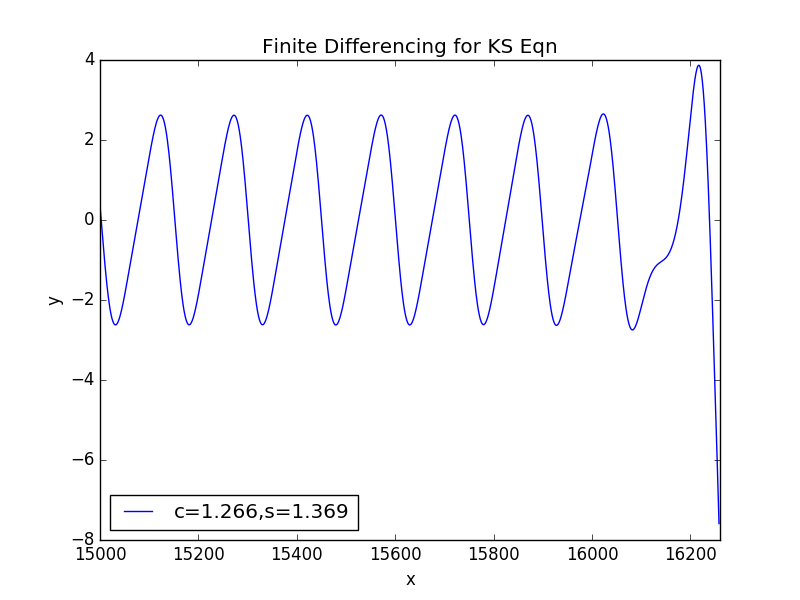
\includegraphics[scale=0.5]{ACxyplotc1266s1369a.png}
  \caption{
$(xy)$ plot. The trajectory generated through a finite difference scheme
outlined in Michelson\rf{Mks86} for $c=1.266$ and $s=1.369$.
  }

  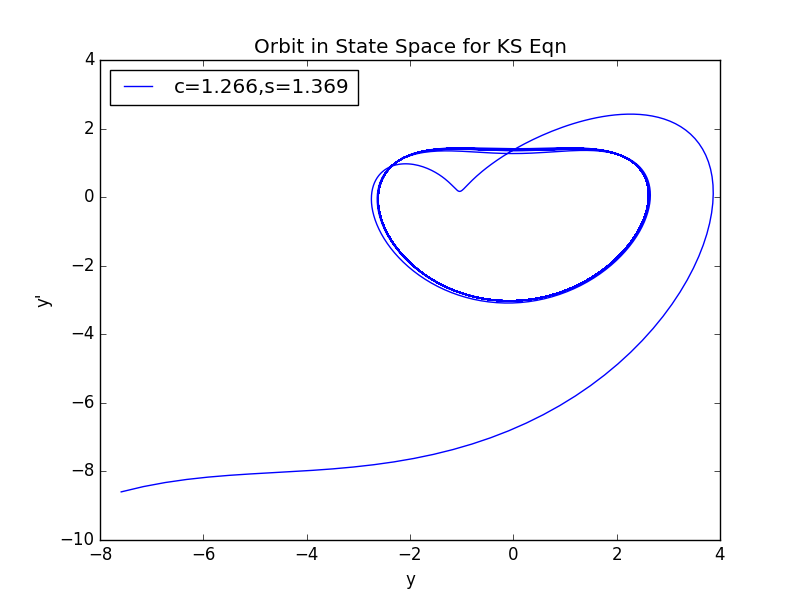
\includegraphics[scale=0.5]{ACorbitc1266s1369a.png}
  \caption{\Statesp\ plot. The near-periodic orbit generated through a finite difference
  scheme outlined in Michelson\rf{Mks86} for $c=1.266$ and $s=1.369$.}
\end{figure}
}

\PCpost{2017-10-23}{
For whatever that is worth, my lecture on the equilibria of \KS\ is
                                                    \toVideo{youtu.be/9ng_yENhXEs}
\HREF{https://www.youtube.com/embed/9ng_yENhXEs} {here}.
    }


\item[2016-01-12 PC]  Literature
related to Michelson\rf{Mks86}:

Carmona \etal\rf{CFGT15}
{\em Noose structure and bifurcations of periodic orbits in reversible
three-dimensional piecewise linear differential systems}

Barker \etal\rf{BJNRZ12}
{\em Stability of periodic { Kuramoto-Sivashinsky} waves}

Aderogba, A. A. and Chapwanya, M. and Djoko\rf{AdChDj12}
{\em Travelling wave solution of the {Kuramoto-Sivashinsky} equation: A
computational study}


Dumortier,  Ibanez  and Kokubu\rf{DuIbKo06}
{\em Cocoon bifurcation in three-dimensional reversible vector fields}

Heidel and Zhang\rf{HeiZha07}
{\em Nonchaotic and chaotic behavior in three-dimensional quadratic systems:
{Five}-one conservative cases},

Nickel\rf{Nickel07}
{\em Travelling wave solutions to the {Kuramoto–Sivashinsky} equation }

Blomgren, Gasner, and Palacios\rf{BlGaPa05}
{\em Hopping behavior in the Kuramoto–Sivashinsky equation}
seems to be specific to $2D$: `` numerical `hopping' cellular flame
patterns are characterized by nonuniform rotations of a ring of cells, in
which individual cells make abrupt changes in their angular positions
while they rotate around the ring. Until now, these states have been
observed only in experiments but not in truly two-dimensional computer
simulations. A modal decomposition analysis of the simulated patterns,
via the proper orthogonal decomposition, reveals spatiotemporal behavior
in which the overall temporal dynamics is similar to that of equivalent
experimental states but the spatial dynamics exhibits a few more features
that are not seen in the experiments.
''


Dumortier,  Ibanez  and Kokubu\rf{DuIbKo06}
{\em Cocoon bifurcation in three-dimensional reversible vector fields}

Rempel \etal\rf{RCMR04}
{Analysis of chaotic saddles in high-dimensional dynamical systems: the
{Kuramoto-Sivashinsky} equation}: ``
study the role played by nonattracting chaotic sets called chaotic
saddles in chaotic transitions of high-dimensional dynamical systems. Our
methodology is applied to the Kuramoto-Sivashinsky equation. The paper
describes a novel technique that uses the stable manifold of a chaotic
saddle to characterize the homoclinic tangency responsible for an
interior crisis, a chaotic transition that results in the enlargement of
a chaotic attractor. The numerical techniques explained here are
important to improve the understanding of the connection between
low-dimensional chaotic systems and spatiotemporal systems which exhibit
temporal chaos and spatial coherence.''

Wilczak\rf{Wilczak03}
{\em Chaos in the {Kuramoto-Sivashinsky} equations -- a computer-assisted proof}

Strauss and Wang\rf{StrWan02}
 {\em Instability of traveling waves of the {Kuramoto-Sivashinsky} equation}

Ishimura\rf{Ishimura02}
{\em Remarks on third-order {ODEs} relevant to the {Kuramoto-Sivashinsky} equation}

Ishimura and Nakamura\rf{IshNak00}
{\em Nonexistence of monotonic solutions of some third-order ode relevant
to the {Kuramoto-Sivashinsky} equation}

Wittenberg and Holmes\rf{witt99hol}
{\em Scale and space localization in the {Kuramoto-Sivashinsky} equation}:
  ``
Using a wavelet basis, the spatiotemporally chaotic regime of the
    KSe is explored where a good seperation of scales is observed. In
    large scales, the dynamics is Gaussian. In the intermediate scales,
    the dynamics is reminiscent of travelling waves and heteroclinic
    cycles which is the typical behavior for small system size. In the
    small scales, the dynamics is intermittent. Through investigation
    of the interaction between different scales, we see the intermediate
    structures give the defining shape of the cell and the large scales
    trigger the spatiotemporal chaos. The small scales dissipate energy
    and modify the background in a average sense.

Yang\rf{ksyang97}
{\em On travelling-wave solutions of the {Kuramoto-Sivashinsky} equation}


Lau\rf{lau92}
{\em The cocoon bifurcations in three-dimensional systems with two fixed points}

Jones, Troy and MacGillivary\rf{kstroy92}
{\em Steady solutions of the {Kuramoto-Sivashinsky} equation for small wave speed}

Grimshaw and Hooper\rf{ksgrim91}
{\em The non-existence of a certain class of travelling wave solutions of
the {Kuramoto-Sivashinsky} equation},

Troy\rf{kstroy89}
{\em The existence of steady solutions of the {Kuramoto-Sivashinsky} equation}

Hooper and Grimshaw\rf{kshooper88}
{\em Travelling wave solutions of the {Kuramoto-Sivashinsky} equation}

Stanislavova and Stefanov\rf{StaSte11}
{\em Asymptotic estimates and stability analysis of {Kuramoto-Sivashinsky}
type models}

\end{description}

\subsection{Dong and Lan / DoLa14}
\label{sect:DoLa14}
Dong and Lan\rf{DoLa14}
{\em Organization of spatially periodic solutions of the steady
{Kuramoto-Sivashinsky} equation}

\begin{description}

\MNGpost{2017-07-17}{
{\bf DoLa14}
The goal of Dong and Lan\rf{DoLa14}
% {\em Organization of spatially
% periodic solutions of the steady {Kuramoto-Sivashinsky} equation}
is to
formulate a systematic way to locate periodic orbits with variational
method developed by Lan  and Cvitanovi{\'c}\rf{CvitLanCrete02,lanVar1},
as well as develop symbolic dynamics to classify these periodic orbits.
    }

\item[2013-12-29 PC] Dong and Lan\rf{DoLa14} study \eqva\ of \KS\ at $L
    = 43.5$. Previous system sizes were  was for antisymmetric
    subspace, system size $ \tildeL = 2.89109$ in
    \refref{Christiansen97}, $L = 38.5$ in \refref{lanCvit07}, $L =
    40.95$ in Lan~\etal\rf{LCC06}, and full \statesp\ $L=22$ in
    \refref{SCD07}. Dong and Lan continue the discussion of Lan's
    \HREF{http://www.cns.gatech.edu/~y-lan/thesis/thesis.pdf}
    {thesis}\rf{LanThesis}. Only \eqva, no mention of \reqva.

They credit Troy\rf{kstroy89,kstroy92} and Greene \& Kim\rf{ksgreene88}
with first studies of \KS\ \eqva.

\ACpost{2017-11-01}{{\bf DoLa14}
Reading this paper's introduction and background tremendously helped me understand
the \KSe\ more.
\begin{equation}
    u_t = (u^2)_x - u_{xx} - \nu u_{xxxx}
\end{equation}
The first derivative term is responsible for the interactions
between spatial modes at different scales (assuming this means length scales $L$)
and transfers energy from the low wavenumber modes to the higher ones. The second
term pumps energy into the system and makes it unstable at large scales while the
third term dissipates energy and damps at small scales.

Matt has gone over the spectral decomposition of the solution many times, but I
will just repeat it here for reference: using the form
\begin{equation}
    u(x,t) = i \sum_{k=-\infty}^{+\infty} a_k(t) e^{ikqx} \qquad \text{where } q = 2\pi/L,
\end{equation}
we can obtain an infinite ladder of coupled ODEs
\begin{equation}
    \dot{a}_k = [(kq)^2 - \nu (kq)^4] a_k - kq \sum_{m=-\infty}^{+\infty} a_m a_{k-m}.
\end{equation}
Since the dissipation term $\nu (kq)^4$ dominates for large wavenumber components, these
terms will not be excited enough significantly contribute to the dynamics. Thus, we can
truncate the set of ODEs such that $a_k = 0$ for $|k|>N$. In most cases, we take $N = 16$.
For small $L$, all Fourier modes are linearly stable, but the system quickly becomes
increasingly turbulent once $L$ increases by a significant amount.

From the video that Predrag recommended as well as the paper, the \KSe\ can be written as
\begin{align}
    &u^2 - u_x - \nu u_{xxx} = c\\
    &\implies \left\{
    \begin{array}{l}
	u_x = v\\
	v_x = w\\
	w_x = u^2 - v - c
    \end{array}
    \right.\\
    &\implies (u+w)_x = u^2 - c
\end{align}
We can see that $u+w$ increases without bound when $c<u^2$. When $c>u^2$ we can find
attractors appear in the state space. However, something weird happens when $c = u^2$
such that the derivative on the left side of Eqn 4.10 equals 0: both an attractor and
repeller appear in the state space, and it seems that trajectory enters the sink and
reappears at the source (if I'm understanding Predrag's drawing in the video correctly).

I'm still working through the variational methods part of the paper to see what they
actually did with the numerical simulations. So far, it seems that there exists four
simple building blocks for creating allowable orbits. This numbering notation reminds
me of the billiard (or pinball) orbit example that was covered in the Group Theory
class.
}

\item[2013-12-29 PC] we still have to study
Dong and Y. Lan\rf{DoLa14a}
{\em A variational approach to connecting orbits in nonlinear dynamical systems }

\end{description}

`` At fixed system size $L =43.5$, important equilibria
      are identified and shown to organize the dynamics. The first
      integral of the steady KSe leads to a 3D dynamical system with an
      integration constant $c$. At a typical value of $c = 0.40194$, four
      simplest cycles are identified and used as basic building blocks to
      construct longer cycles. The symbolic dynamics based on trajectory
      topology are very effective in classifying all short periodic
      orbits. The the return map on a chosen {\PoincSec} shows the
      complexity of the dynamics and the bifurcation of building blocks
      provides a chart to look for possible cycles at given periods. ''

The $n$ cell state\rf{FSTks86} is stable in finite windows for
arbitrarily large system sizes.

``
the antisymmetric heteroclinic orbit $\in \bbU^+$ connecting the two \eqva\ in
(9) is the only bounded nonconstant solution when the integration
constant $c\to\infty$\rf{mcord86}. For $c$ large enough, the heteroclinic
orbit remains the unique bounded solution\rf{Mks86}. It continues to be
numerically observable with $c$ down to 0.07\rf{kshooper88}, and was
computed analytically with normal form analysis for $c\ll
1$\rf{kschang86}. When $c$ decreases from large values, new connections
with more zeroes are born through saddle-node bifurcations until one
periodic orbit emerges as a limit of the connecting orbit with infinite
number of zeros. Bifurcation analysis with spatial Fourier modes gives
interesting features of spatially periodic steady solutions in certain
parameter regime\rf{ksgreene88}.
''

%%%%%%%%%%%%%%%%%%%%%%%%%%%%%%%%%%%%%%%%%%%%%%%%
\printbibliography[heading=subbibintoc,title={References}]
